%---------------------------------------------------------------------------%
%---------------------------------------------------------------------------%
%                          MPT THEME - EXAMPLE                              %
%---------------------------------------------------------------------------%
%---------------------------------------------------------------------------%

%---------------------------------------------------------------------------%
% HEADER                                                                    %
%---------------------------------------------------------------------------%

%----- DOCUMENT TYPE--------------------------------------------------------%
%---------------------------------------------------------------------------%

\pdfminorversion = 5
\documentclass[10pt]{beamer}
\usetheme[francais %[For documents written in french]
%,notocfoot %[To remove the presentation title in the footer of the frames]
%,arial %[To use arial as the default text font instead of Linux Biolinum]
,alertred %[For the alterted text to be framed in red instead of blue]
%,euler %[To use euler as the default math font instead of XITS]
%,sober %[To remove the grey areas behind the frame titles and the footer]
]{MPTM} %[Comment and uncomment options as desired]


%----- PACKAGES-------------------------------------------------------------%
%---------------------------------------------------------------------------%
% [Put all desired packages here]

%Notes
\usepackage{pdfpages}
%\setbeameroption{show notes} %[to show note on the pdf]
%\setbeameroption{show notes on second screen=right}%Pour placer les notes à droite, en extension d'une slide mais commande qui ne marche pas


%TIKZ
\usepackage{pgfplots}

\pgfplotsset{compat=1.14}

\usetikzlibrary{calc, 3d, positioning, intersections, backgrounds, shapes, math, shapes.geometric, topaths, decorations.markings, pgfplots.colormaps}
\usepgfplotslibrary{colormaps, fillbetween}
\pgfplotsset{probastyle/.style={smooth, width = \textwidth, axis x line = bottom, axis y line = left,
		every axis x label/.style={ at={(ticklabel* cs:1.05)}, anchor=west,},
		every axis y label/.style={	at={(ticklabel* cs:1.05)}, anchor=south,}}}
\pgfplotsset{ colormap={MPT}{rgb255(0cm)=(0,94,158) rgb255(0.25cm)=(0,111,182) rgb255(1cm)=(240,240,240) rgb255(2cm)=(156,158,159)}}
\pgfplotsset{compat=newest}
\pgfplotsset{school/.style={tick align = outside, major tick length = 2.5pt, axis line style={-stealth}, anchor = center, x label style = {anchor = west, at = {(current axis.right of origin)}}, y label style = {anchor = south, at = {(current axis.above origin)}, rotate = -90}}}
\usepackage{tikz-3dplot}
\tdplotsetmaincoords{60}{-30}
\tdplotsetrotatedcoords{0}{90}{90}
\pgfmathdeclarefunction{gaussShape}{2}{%
  \pgfmathparse{(1/#2)*exp(-((x-#1)^2)/(1^2))}%
  }
  \pgfmathdeclarefunction{gauss}{2}{%
  \pgfmathparse{(1/(#2*sqrt(2*pi)))*exp(-((x-#1)^2)/(2*#2^2))}%
}
\tikzset{
		    base/.style = {draw=MPTgrey, ultra thick, 
			minimum height=30mm, minimum width=30mm,
			inner sep=0pt}, %permet d'afficher une image dans un rectangle
  invisible/.style={opacity=0},
  visible on/.style={alt={#1{}{invisible}}},
  alt/.code args={<#1>#2#3}{%
    \alt<#1>{\pgfkeysalso{#2}}{\pgfkeysalso{#3}} % \pgfkeysalso doesn't change the path
  },
}
\usetikzlibrary{arrows.meta}

%smiley souriant bleu
\newcommand{\smiley}{\tikz[baseline=-0.75ex,black]{
		\draw[MPTblue] circle (2mm);
		\node[MPTblue,fill,circle,inner sep=0.5pt] (left eye) at (135:0.8mm) {};
		\node[MPTblue,fill,circle,inner sep=0.5pt] (right eye) at (45:0.8mm) {};
		\draw[MPTblue] (-145:0.9mm) arc (-120:-60:1.5mm);
	}
}

%smiley pas content rouge
\newcommand{\frownie}{\tikz[baseline=-0.75ex,black]{
		\draw[MPTred] circle (2mm);
		\node[MPTred,fill,circle,inner sep=0.5pt] (left eye) at (135:0.8mm) {};
		\node[MPTred,fill,circle,inner sep=0.5pt] (right eye) at (45:0.8mm) {};
		\draw[MPTred](-145:0.9mm) arc (120:60:1.5mm);
	}
}


%----- MATH
%\usepackage{amsmath, amssymb, amscd, latexsym, bigints, stmaryrd, bm}
\usepackage{stmaryrd, bm}

%----- TABLES
\usepackage{booktabs, tabularx, multirow, colortbl}
\arrayrulecolor{main}
\setlength{\aboverulesep}{0pt}
\setlength{\belowrulesep}{0pt}
\setlength{\extrarowheight}{5pt}
\newcolumntype{L}{>{\raggedright\arraybackslash}X}
\newcolumntype{R}{>{\raggedleft\arraybackslash}X}
\newcolumntype{C}{>{\centering\arraybackslash}X}
\newcolumntype{s}{@{\hspace{3pt}} c @{\hspace{6pt}}}

%----- FIGURES
\usepackage{graphicx, psfrag, color, epsfig}   % to include and manipulate graphics
\usepackage[all]{xy}    % to draw diagrams
%\usepackage{ifsym}
\usepackage{multirow}

%----- LISTS
\usepackage{enumerate}

%----- BIBLIO
\usepackage{bibentry}

%-----BARRER
\usepackage{soul}

%----- SYMBOLS
\usepackage{pifont}
\usepackage{bclogo}

%----Font
\usepackage{verbatim}
\usepackage{fancyvrb}
\makeatletter
\newcommand{\verbatimfont}[1]{\renewcommand{\verbatim@font}{\ttfamily#1}}
\makeatother

%\usepackage{secdot}
%\sectiondot{subsection}

%----- ADDITIONAL COMMANDS 
%---------------------------------------------------------------------------
\newcommand{\bfun}{\bm{1}}
%\let\sectionOld\section
%\renewcommand\section[2][\empty]{%boldmath\sectionOld[#1]{#2}\unboldmath%}
% [Put all user-defined commands here]

%----- Symbols
\newcommand{\ex}{{\color{MPTblue}\ding{228}}}
%\newcommand{\ex}{{\color{MPTblue}\small{\blacktriangleright}}}

%----- SPACES
\newcommand{\hsp}{\hspace*{1em}}
\newcommand{\midhsp}{\hspace*{.5em}}

\makeatletter
\define@key{beamerframe}{c}[true]{% centered
	\beamer@frametopskip=0pt plus 1fill\relax%
	\beamer@framebottomskip=0pt plus 1fill\relax%
	\beamer@frametopskipautobreak=0pt plus .4\paperheight\relax%
	\beamer@framebottomskipautobreak=0pt plus .6\paperheight\relax%
	\def\beamer@initfirstlineunskip{}%
}
\makeatother



%----- BIBLIO
\newcommand{\itbib}[1]{{\itshape \bibentry{#1}}}
%\providecommand{\bysame}{S.I. Resnick}%

%----- PATHS
%---------------------------------------------------------------------------%
\graphicspath{{Images/}}	%[Indicate the name of the file where your images are stored]

%---------------------------------------------------------------------------%
% TITLE                                                                     %
%---------------------------------------------------------------------------%

\title{Apprentissage supervisé et non supervisé}
\subtitle{
	{}}
\author{}
%\institute{Mines ParisTech}{Equipe Géostatistique}{}
%\coauthor{Sophie Lèbre}
%\coauthor[2]{Anne Sabourin}
%\coinstitute{Mines ParisTech}{Equipe Géostatistique}{}
%\coinstitute[2]{Telecom Paris}{Equipe S2A}{}
\date{}
\event{M1 MIASHS}
%\subtitle{Subtitle}
\rclogo{}	% Research center(s) logo(s)
\netlogo{}	% Partner(s)  logo(s) separated by comma

%---------------------------------------------------------------------------%
% PRESENTATION                                                              %
%---------------------------------------------------------------------------%
\begin{document}
	
%---------------------------------------------------------------------------%
% TITLE FRAME                                                               %
%---------------------------------------------------------------------------%
\begin{frame}
	\maketitle
\end{frame}

%---------------------------------------------------------------------------%
% TOC SETUP                                                                 %
%---------------------------------------------------------------------------%

%Ce qui est affiché quand on a la commande \section{}

\AtBeginSection[]{
	{
		\usebackgroundtemplate{
			\begin{tikzpicture} [inner sep = 0pt, outer sep = 0pt]
			
			%----- MASK - \pgflinewidth
			\node [anchor = north west, minimum width = \paperwidth - \pgflinewidth, minimum height = \paperheight - \pgflinewidth] (pc) at (current page.north west) {};
			
			%----- BACKGROUND
			\shade[top color = event.bg, bottom color = white] (pc.north west) rectangle ([yshift = -15pt]pc.north east);
			\shade[bottom color = event.bg, top color = white] (pc.south west) rectangle ([yshift = 15pt]pc.south east);
			
			----- SECTION NUMBER %[Uncomment if you want the section number to appear in the background]
			\node[minimum height = .9\paperheight, anchor = center] at (current page.center) 				 {\color{event.bg}{\fontsize{300}{0}\selectfont \Roman{section}}};
			
			%----- TITLE SECTION
			\node[anchor = center, text centered] at (current page.center) {\begin{minipage}[c]{.9\textwidth} \centering \huge\bfseries\scshape\color{MPTblue}\insertsection
			\end{minipage}};
			
			%%----- BACK/PROB/STAT/ALGO %pour rajouter des logos sur la page de section
			%\node[anchor = north west] at ([xshift = 1em, yshift = -2em]current page.north west) {
%				\ifnumequal{\value{section}}{1}{
\includegraphics[width = 2cm]{Back.pdf}}{}
			%};
			\end{tikzpicture}
		}
		\begin{frame}[noframenumbering, plain]
			
		\end{frame}
	}
}


%Ce qui est affiché quand on a la commande \subsection{}
\AtBeginSubsection[]{
	{
		\usebackgroundtemplate{
			\begin{tikzpicture} [inner sep = 0pt, outer sep = 0pt]
				
				%----- MASK - \pgflinewidth
				\node [anchor = north west, minimum width = \paperwidth - \pgflinewidth, minimum height = \paperheight - \pgflinewidth] (pc) at (current page.north west) {};
				
				%----- BACKGROUND
				\shade[top color = event.bg, bottom color = white] (pc.north west) rectangle ([yshift = -15pt]pc.north east);
				\shade[bottom color = event.bg, top color = white] (pc.south west) rectangle ([yshift = 15pt]pc.south east);
				
				----- SECTION NUMBER %[Uncomment if you want the section number to appear in the background]
				\node[minimum height = .9\paperheight, anchor = center] at (current page.center)
				{\color{event.bg}{\fontsize{300}{0}\selectfont\Roman{section}}};

			
			%----- TITLE SUBSECTION
			\node[anchor = center, text centered] (sub) at (
			%[yshift = - \insep-1.8cm]
			current page.center) {\begin{minipage}[c]{.9\textwidth} \centering
			\LARGE\bfseries\scshape\color{MPTgrey}\Alph{subsection}.
			\insertsubsection
			\end{minipage}};
		\node[text centered] at ([yshift =  50]sub.north) {\begin{minipage}[c]{.9\textwidth} \centering
				\huge\bfseries\scshape\color{MPTblue}\insertsection
		\end{minipage}};
							\end{tikzpicture}
		}
		\begin{frame}[noframenumbering, plain]
			
		\end{frame}
	}
}

%Ce qui est affiché quand on a la commande \subsubsection{}
\AtBeginSubsubsection[]{
	{
		\usebackgroundtemplate{
			\begin{tikzpicture} [inner sep = 0pt, outer sep = 0pt]
				
				%----- MASK - \pgflinewidth
				\node [anchor = north west, minimum width = \paperwidth - \pgflinewidth, minimum height = \paperheight - \pgflinewidth] (pc) at (current page.north west) {};
				
				%----- BACKGROUND
				\shade[top color = event.bg, bottom color = white] (pc.north west) rectangle ([yshift = -15pt]pc.north east);
				\shade[bottom color = event.bg, top color = white] (pc.south west) rectangle ([yshift = 15pt]pc.south east);
				
				----- SECTION NUMBER %[Uncomment if you want the section number to appear in the background]
				\node[minimum height = .9\paperheight, anchor = center] at (current page.center)
				{\color{event.bg}{\fontsize{300}{0}\selectfont\Roman{section}}};
				
				
				%----- TITLE SUBSECTION
				\node[anchor = center, text centered] (subsub) at (
				%[yshift = - \insep-1.8cm]
				current page.center) {\begin{minipage}[c]{.9\textwidth} \centering \Large\bfseries\scshape\color{black!70!white}\arabic{subsubsection}. 
						\insertsubsubsection
				\end{minipage}};
						\node[text centered] (sub) at ([yshift =  40]subsub.north) {\begin{minipage}[c]{.9\textwidth} \centering
					\LARGE\bfseries\scshape\color{MPTgrey}\Alph{subsection}.
					\insertsubsection
			\end{minipage}};
			\node[text centered] at ([yshift =  30]sub.north) {\begin{minipage}[c]{.9\textwidth} \centering
					\huge\bfseries\scshape\color{MPTblue}\insertsection
			\end{minipage}};
			\end{tikzpicture}
		}
		\begin{frame}[noframenumbering, plain]
			
		\end{frame}
	}
}




%---------------------------------------------------------------------------%
% INTRODUCTION                                                              %
%---------------------------------------------------------------------------%
%
%---------------------------------------------------------------------------%
%
%
%---------------------------------------------------------------------------%
%


%\begin{frame}[fragile, noframenumbering]
%	\bftitle{Intervenantes}\hspace{1.7em}  Sophie Lèbre, Marine Demangeot\\[3em]
%	\bftitle{5 cours} \hspace{5em} mercredi 21 septembre \hspace{0.3em} \textcolor{MPTgrey}{(9h00-12h15)} \hfill \\[0.2em]
%	\phantom{\bftitle{5 cours} }  \hspace{5em} jeudi 22 septembre \hspace{1.6em} \textcolor{MPTgrey}{(9h00-12h15)} \hfill \\[0.2em]
%	\phantom{\bftitle{5 cours} }  \hspace{5em} lundi 10 octobre \hspace{2.8em} \textcolor{MPTgrey}{(9h00-12h15)} \hfill \\[0.2em]
%	\phantom{\bftitle{5 cours} }   \hspace{5em} lundi 17 octobre \hspace{2.4em} \textcolor{MPTgrey}{(14h00-17h15)} \hfill \\[0.2em]
%	\phantom{\bftitle{5 cours} }  \hspace{5em} jeudi 20 octobre \hspace{2.4em} \textcolor{MPTgrey}{(14h00-17h15)} \hfill \\[3em]
%	%
%	\bftitle{Logiciel} \hspace{5em}  \verbatimfont{\large} \verb|R|
%	\phantom{l}\\[3em]
%	
%	\bftitle{Examen} \hspace{5em} vendredi 18 novembre \textcolor{MPTgrey}{(10h15-12h15) } \hfill \\
%	\phantom{\bftitle{Examen}} \hspace{5em} examen sur papier, sans documents
%	
%%-------------------------NOTES-------------------------------
%\note{N'oublie pas que tu peux rajouter des notes}
%%-------------------------------------------------------------	
%\end{frame}

%------------------------------------------------------------------------------------------
%------------------------------------------------------------------------------------------

%\begin{frame}
%	\begin{center}
%	\large\textcolor{MPTblue}{Ce cours s'inspire très largement de l'ouvrage\\[0.5em] \textit{\href{http://cazencott.info/dotclear/public/lectures/IntroML_Azencott.pdf}{Introduction au Machine Learning}} \\[0.5em] de Chloé-Agathe Azencott} 
%	\end{center}
%\end{frame}
%------------------------------------------------------------------------------------------
%------------------------------------------------------------------------------------------

\section*{Introduction}

\section*{L'apprentissage supervisé}

%------------------------------------------------------------------------------------------
%------------------------------------------------------------------------------------------

\subsection*{Cadre de l'apprentissage supervisé}

\subsection*{La régression logistique}



%
%\begin{frame}
%	\begin{tikzpicture} [inner sep = 0pt, outer sep = 0pt]
%		
%		%----- MASK - \pgflinewidth
%		\node [anchor = north west, minimum width = \paperwidth - \pgflinewidth, minimum height = \paperheight - \pgflinewidth] (pc) at (current page.north west) {};
%		
%		%----- BACKGROUND
%		\shade[top color = event.bg, bottom color = white] (pc.north west) rectangle ([yshift = -15pt]pc.north east);
%		\shade[bottom color = event.bg, top color = white] (pc.south west) rectangle ([yshift = 15pt]pc.south east);
%		
%	%
%		
%		%----- TITLE SECTION
%		\node[anchor = center, text centered] at (current page.center) {\begin{minipage}[c]{.9\textwidth} \centering \huge\bfseries\scshape\color{MPTblue}\insertsection
%		\end{minipage}};
%		
%		%%----- BACK/PROB/STAT/ALGO %pour rajouter des logos sur la page de section
%		%\node[anchor = north west] at ([xshift = 1em, yshift = -2em]current page.north west) {
%			%				\ifnumequal{\value{section}}{1}{
\includegraphics[width = 2cm]{Back.pdf}}{}
%			%};
%	\end{tikzpicture}
%\end{frame}
%------------------------------------------------------------------------------------------
%------------------------------------------------------------------------------------------



%------------------------------------------------------------------------------------------
%------------------------------------------------------------------------------------------


%------------------------------------------------------------------------------------------
%------------------------------------------------------------------------------------------


\subsection{Les arbres de décisions}

\begin{frame}
	Les modèles étudiés jusqu'ici, principalement les KNN et la régression logistique, réalisent l'étiquetage d'un observation $x \in \X$ en une seule étape. En particulier, ils utilisent le même ensemble de variables pour toutes les classes, et leur accordent la même importance pour toutes les observations.\\[1em]
	
	Ce n'est donc pas adapté aux situations où les classes ont une distribution multimodale, suivant les régions de l'espace considérées,  elles sont déterminées par différentes variables. \\
	\textcolor{MPTgrey}{ex : symptomes d'une maladie qui ne sont pas les mêmes suivant l'âge de l'individu.}\\[1em]
	
	Les arbres de décision, au contraire, sont des modèles hiérarchiques qui se comportent comme une série successive de tests conditionnels, dans laquelle chaque test dépend des tests précédents et de leur résultat. 
	
	\note{Dire "livre dont vous êtes le héros". à changer car j'ai paraphraser CHloée azencott}
\end{frame}
%%------------------------------------------------------------------------------------------

\begin{frame}
		\bftitle{Définition}
	\begin{vblock}{}
		On appelle \textit{\bfblue{arbre de décision}} un modèle de prédiction qui peut être représenté sous la forme d’un arbre. Chaque noeud de l’arbre teste une condition sur une seule variable et chacun de ses enfants correspond à une réponse possible à cette condition. Les feuilles de l’arbre correspondent à une étiquette.
	\end{vblock}
	
	
	\begin{center}
		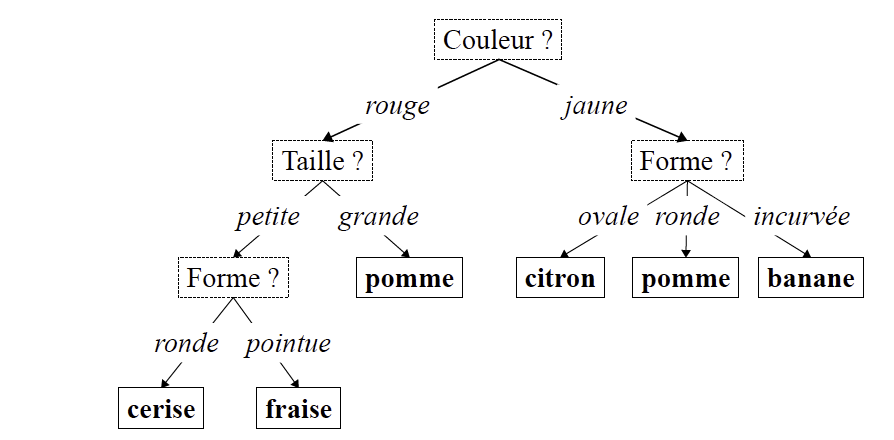
\includegraphics[width=0.8\textwidth,clip]{arbreFruits.png}

\vspace*{1.5em}
\footnotesize{\textcolor{MPTgrey}{Tirée de l'ouvrage \textit{\href{http://cazencott.info/dotclear/public/lectures/IntroML_Azencott.pdf}{Introduction au Machine Learning}} de Chloé-Agathe Azencott} }
	\end{center}
\end{frame}
%
%%------------------------------------------------------------------------------------------
\begin{frame}

	
	\begin{center}
		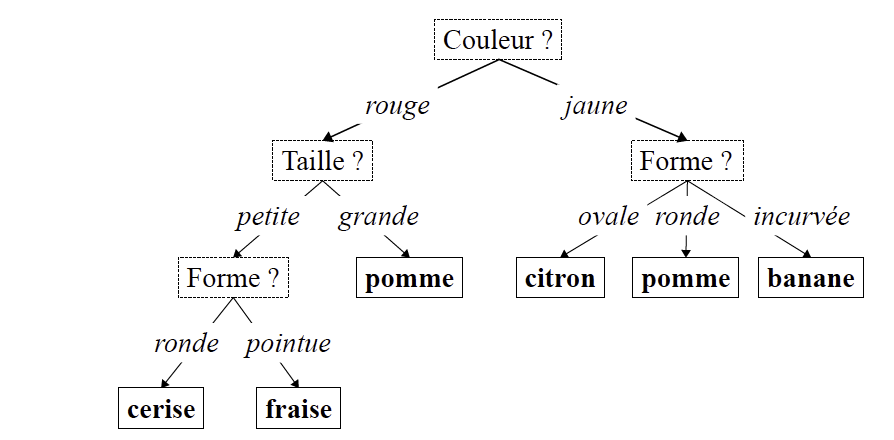
\includegraphics[width=0.5\textwidth,clip]{arbreFruits.png}
		
		\vspace*{1em}
	
	\end{center}
	
	Les arbres de décision \\[1em]
	\begin{itemize}
		\item  permettent de traiter des variables qualitatifs (ex : taille et couleur du fruit), sans nécessiter une représentation numérique de ces variables. On parle \textit{d’apprentissage non métrique}. Ils sont donc adaptés aux données hétérogènes (variables quantitatives et qualitatives)\\[0.7em]
		%une notion de similarité ou d’ordre sur ces attributs (on parle \textit{d’apprentissage non métrique}) ;
		\item permettent de traiter un problème de classification multiclasse sans passer par des classifications binaires \clrcite{Et pour les KNN ? pour la régression logistique ?}\\[0.7em]
		\item  permettent de traiter des classes multi-modales (comme ici pour l’étiquette « pomme », qui est affectée à un fruit grand et rouge ou à un fruit jaune et rond.)
		\clrcite{Et pour les KNN ? pour la régression logistique ?}\\[0.5em]
	\end{itemize}
	
	\note{Donc les arbres de décision sont particulièrement adaptés aux données hétérogènes :
		mélange de variables numériques et catégorielles.
		
		Classes multimodales : et KNN ? et reg logistique ?}
\end{frame}
%
%%------------------------------------------------------------------------------------------


\begin{frame}{L'algorithme CART}
	
	Pour constuire des arbres de décisions, on peut utiliser l'algorithme CART (Classification and Regression Tree). C'est un algorithme de partitionnement de l’espace par une approche gloutonne, récursive et divisive qui permet d'apprendre un \textit{arbre binaire} à partir de données d'apprentissage $(x_1,y_1), \dots, (x_n, y_n) \in \X \times \Y$.\\[2em]
	
	\begin{enumerate}
		\item Chaque noeud sépare linéairement le jeu de données (chaque noeud a exactement deux enfants ; pas de perte de généralité car un arbre peut être ré-exprimé sous la forme d’un arbre binaire)\\[1em]
		\item Pour partitionner les données on n’utilise qu’une seule variable par noeud. Pour des variables numériques, la frontière de décision produite est alors orthogonale à l'axe de cette variable.\\[1em]
		\item Lorsqu’on arrive au feuille, on utilise une règle d’agrégation (vote pour un problème de classification, moyenne pour un problème de régression) pour estimer l'étiquette $y$ d'un point $x \in \X$.
	\end{enumerate}
	
	

	
\end{frame}
%%------------------------------------------------------------------------------------------

\begin{frame}{Séparation linéaire}
	
	Un arbre peut être ré-exprimé sous la forme d’un arbre binaire
\begin{center}
	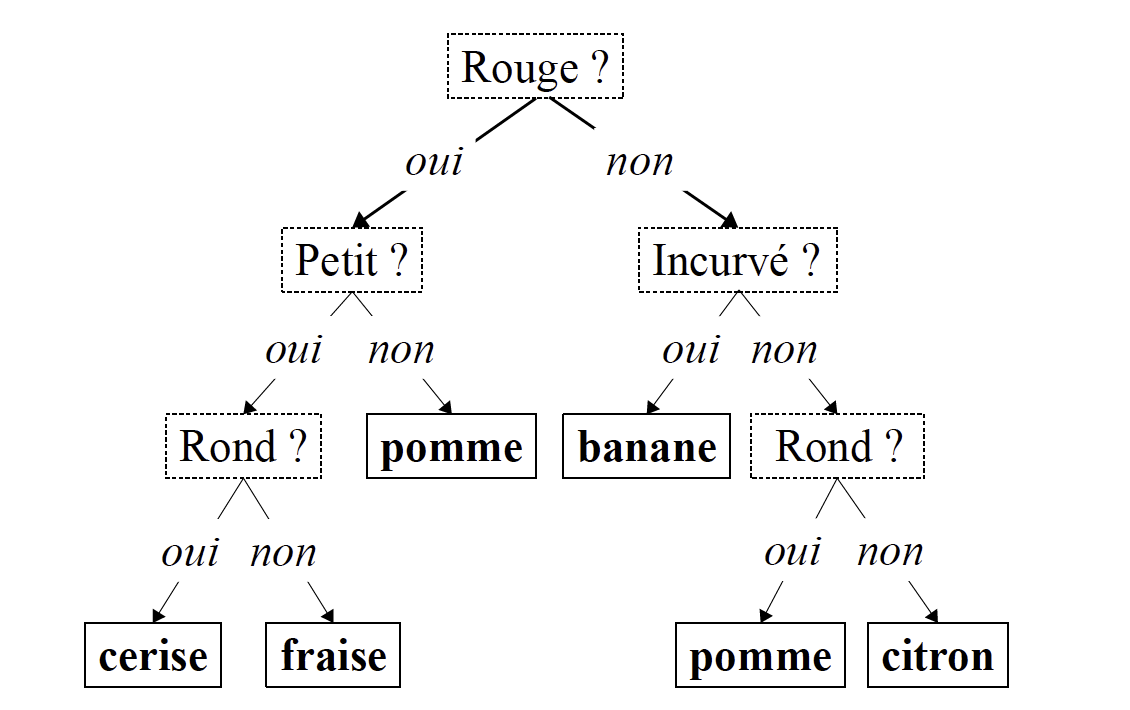
\includegraphics[width=0.65\textwidth,clip]{arbreFruits2.png}
	\vspace*{1.5em}
	
	\footnotesize{\textcolor{MPTgrey}{Tirée de l'ouvrage \textit{\href{http://cazencott.info/dotclear/public/lectures/IntroML_Azencott.pdf}{Introduction au Machine Learning}} de Chloé-Agathe Azencott} }
\end{center}
	
		\vspace*{1.5em}
	\bftitle{Remarque} La construction de l'arbre est itérative, noeud par noeud, en partant de la racine

\end{frame}

%%------------------------------------------------------------------------------------------

\begin{frame}{Une seule variable par noeud}
	
À chaque noeud d’un arbre de décision construit par CART correspond une variable séparatrice $x^j$ selon laquelle vont être partitionnées les données. Cette variable séparatrice définit deux régions $R_{l}$ et $R_{m}$, correspondant aux enfants du noeud considéré.\\[1em]

\bftitle{variable binaire} (quali ou quanti) \,\, Si $x^j$ est binaire alors les deux régions sont
$$ R_l(x^j) = \{ x\in\X : x^j = 1\} \hsp \hsp \hsp  R_m(x^j) = \{ x\in\X : x^j = 0\} $$

\bftitle{variable qualitative nominale}  \,\,  Si $x^j$ peut prendre plus de deux modalités, alors pour un sous-ensemble $\S$ de modalités sélectionnées (souvent $dim(\S)=1$) :
$$ R_l(x^j,\S) = \{ x\in\X : x^j \in \S\} \hsp \hsp \hsp  R_m(x^j,\S) = \{ x\in\X : x^j \notin \S\} $$

\bftitle{variable quantitative continue}  \,\,  Si $x^j$ est une variable quantitative continue, alors pour un point de séparation sélectionné $s$ qui est la valeur de l’attribut par rapport à laquelle va se faire la décision :
$$ R_l(x^j, s) = \{ x\in\X : x^j <s\} \hsp \hsp \hsp  R_m(x^j, s) = \{ x\in\X : x^j \geq s \} $$
	
	
\end{frame}

%%------------------------------------------------------------------------------------------



\begin{frame}{Une seule variable par noeud}
	
	
	\bftitle{variable qualitative ordinale}  \,\, 
 Si $x^j$ est quantitative ordinale, on peut la traiter comme une variable quantitative continue (séparation "par seuil" en respectant l'ordre des modalités) ou comme une variable qualitative nominale (regroupement de modalités) \\[2em]
	
	\bftitle{variable quantitative discrète}  \,\,  Si $x^j$ est une variable quantitative discrète, alors on la traite souvent comme une variable quantitative continue (séparation "par seuil"). Si $x^j$ prend peu de valeurs différentes, on peut aussi la traiter comme une variable qualitative nominale (regroupement de modalités) même si, dans ce cas-là, on perd la notion d'ordre\\[5em]
	
	
\end{frame}

%%------------------------------------------------------------------------------------------



\begin{frame}{Séparation linéaire}
	
Autre exemple 
	\begin{center}
		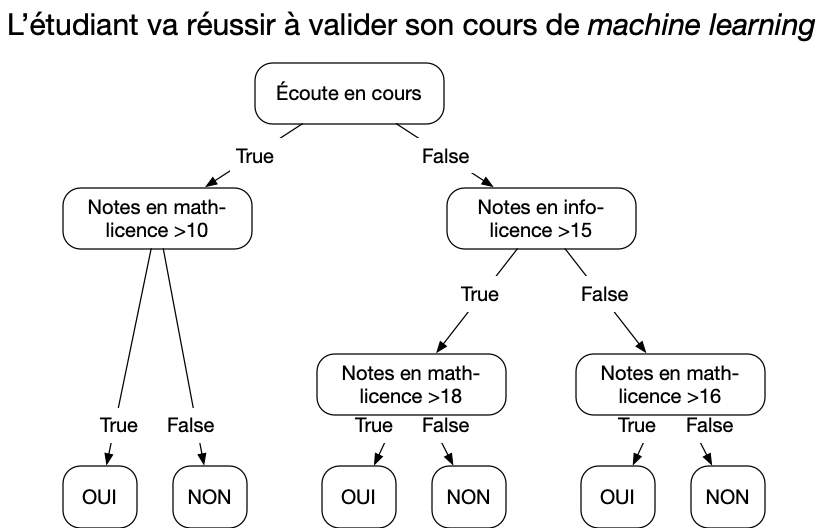
\includegraphics[width=0.8\textwidth,clip]{cart.jpg}
	\end{center}
	
	
	
\end{frame}

%%------------------------------------------------------------------------------------------

\begin{frame}{Une seul variable par noeud }
	
	Notes en maths et en informatique
	\begin{center}
		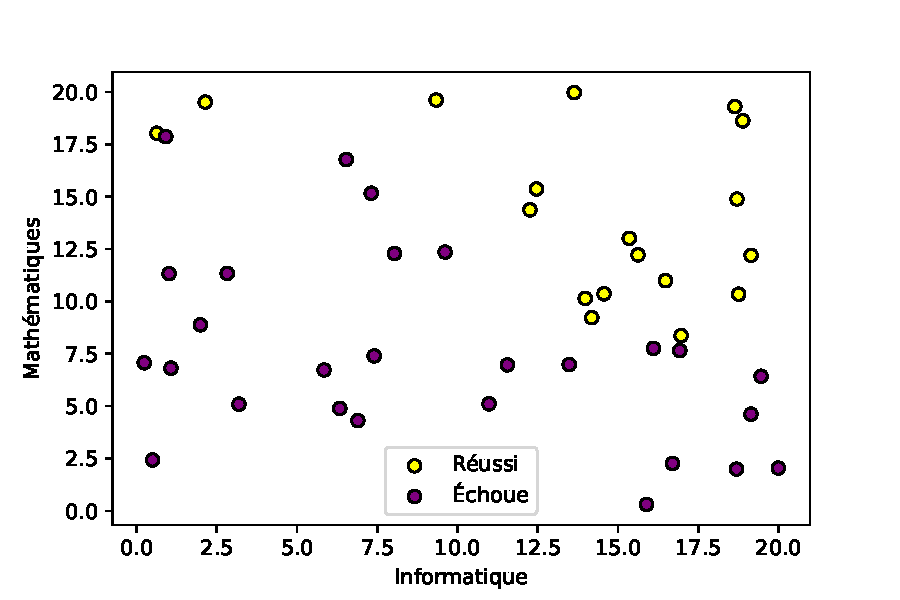
\includegraphics[width=0.8\textwidth,clip]{data_tree.pdf}
	\end{center}
	
	
	
\end{frame}
%%------------------------------------------------------------------------------------------

\begin{frame}{Une seul variable par noeud }
	
	Chaque noeud produit une frontière de décision orthogonale aux axes\\[1.5em]
	\begin{center}
		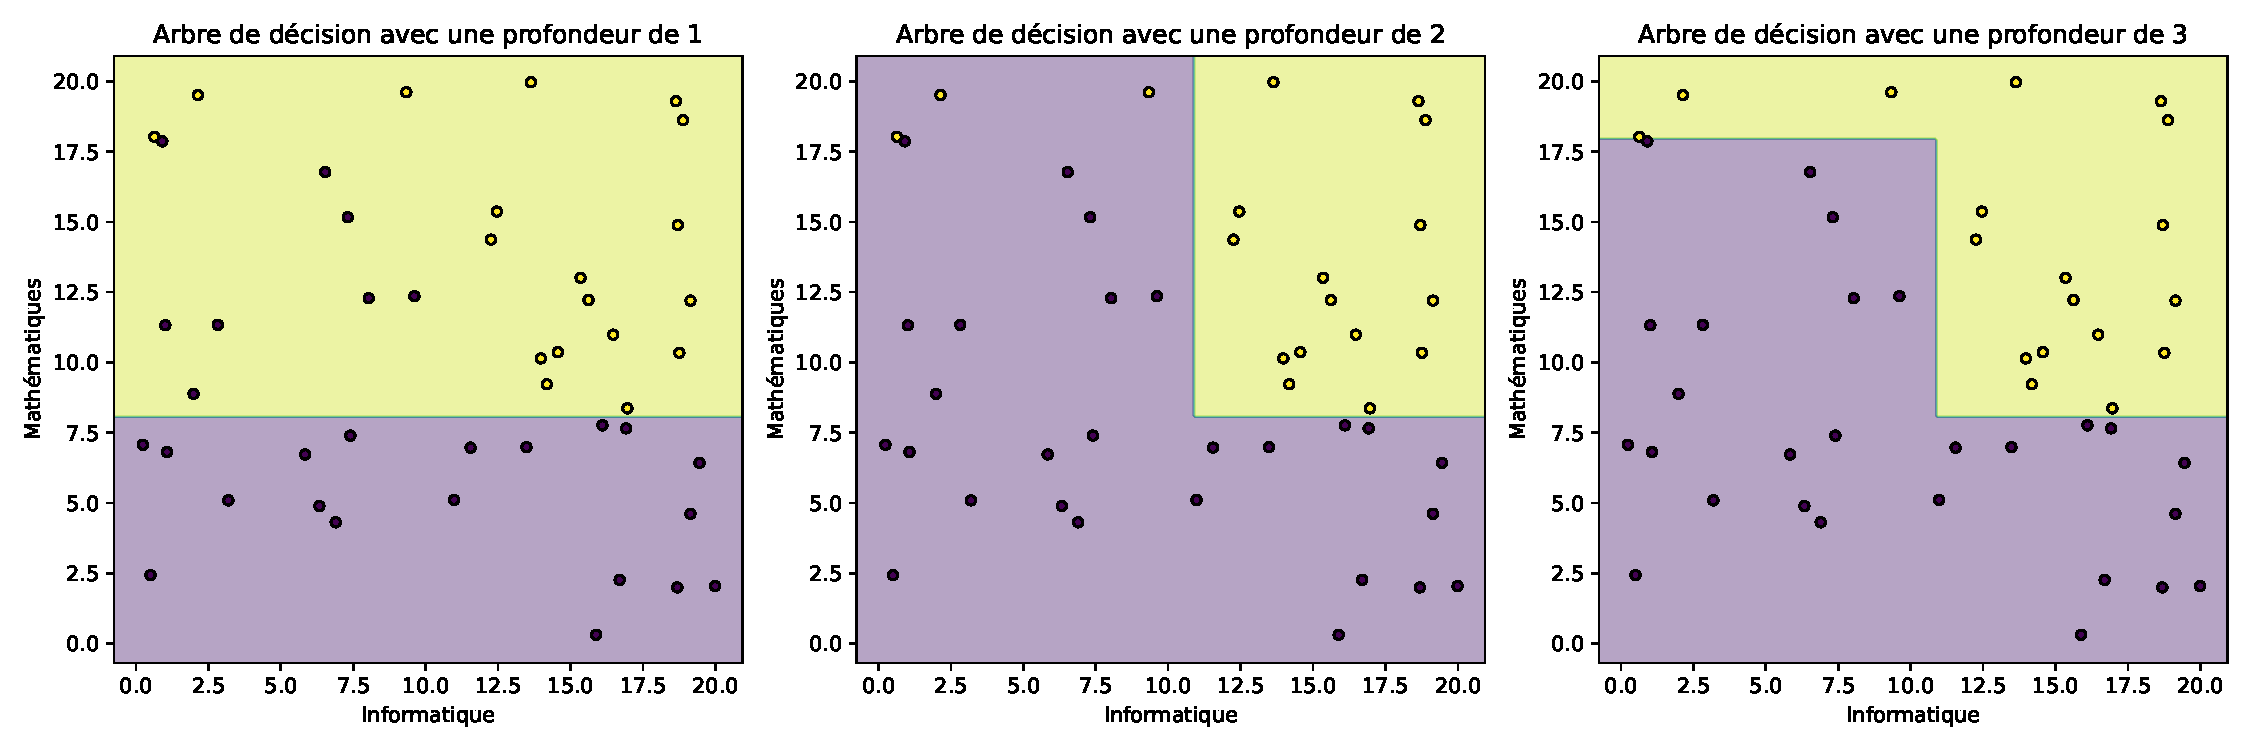
\includegraphics[width=0.9\textwidth,clip]{data_tree_cart.pdf}
	\end{center}
	
	\vspace*{1em}
	
		\bftitle{Remarques}\\[0.5em]
		
		\begin{itemize}
			\item  L'algorithme construit non pas un mais plusieurs séparateurs linéaires pour
			construire des frontières de décision non linéaires.\\[.5em]
			\item Utiliser des séparateurs linéaires parallèles aux axes favorise l'interprétabilité\\[.5em]
			\item Chaque point du jeu de données (et plus généralement, chaque point $x \in \X$) n’appartient qu’à une unique région à un instant donné
		\end{itemize}
		
		
	
\end{frame}

%%------------------------------------------------------------------------------------------

\begin{frame}{Une seul variable par noeud }
	
L'arbre correspondant
	\begin{center}
			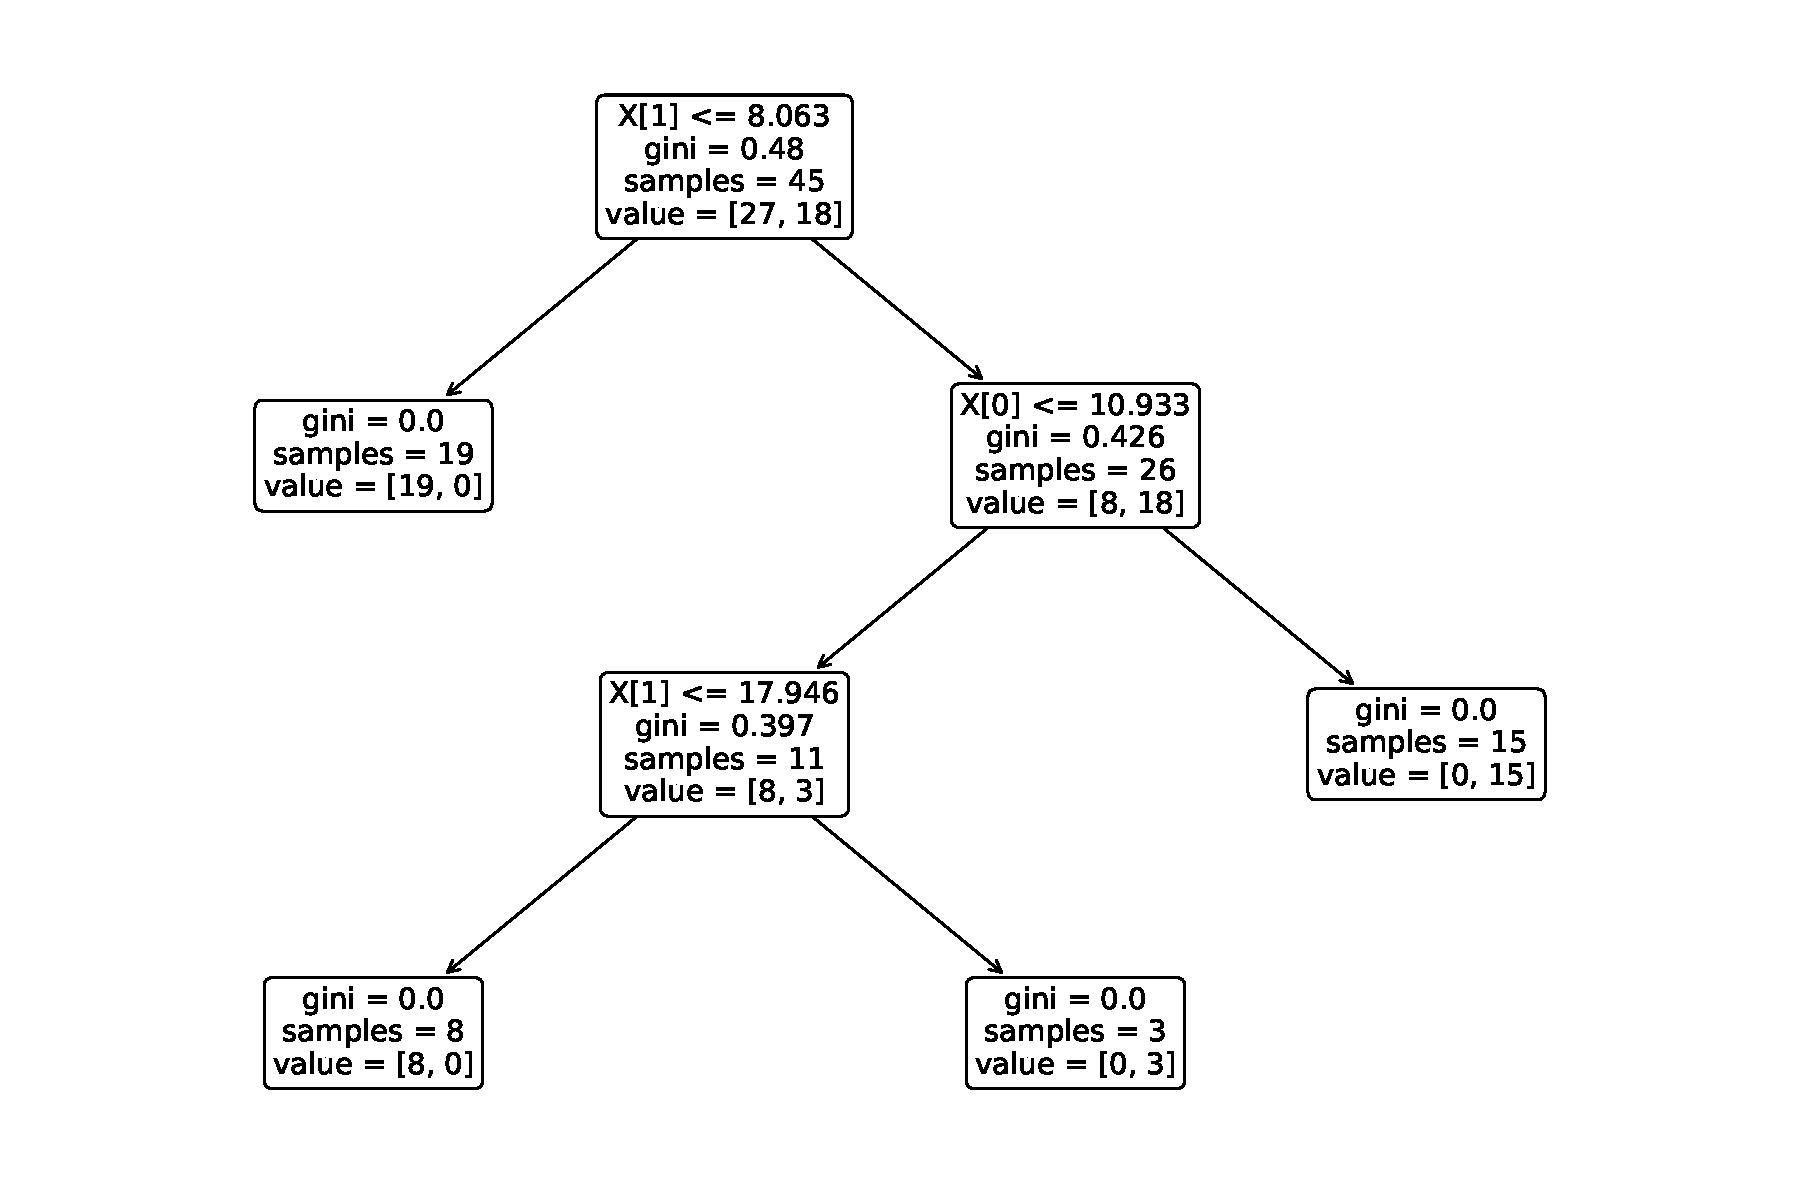
\includegraphics[width=1\textwidth,clip]{the_tree.pdf}
	\end{center}
	
	
	
\end{frame}


%%------------------------------------------------------------------------------------------

\begin{frame}{Une seul variable par noeud }
	
	Quel arbre pour la partition suivante ?
	
	\begin{center}
			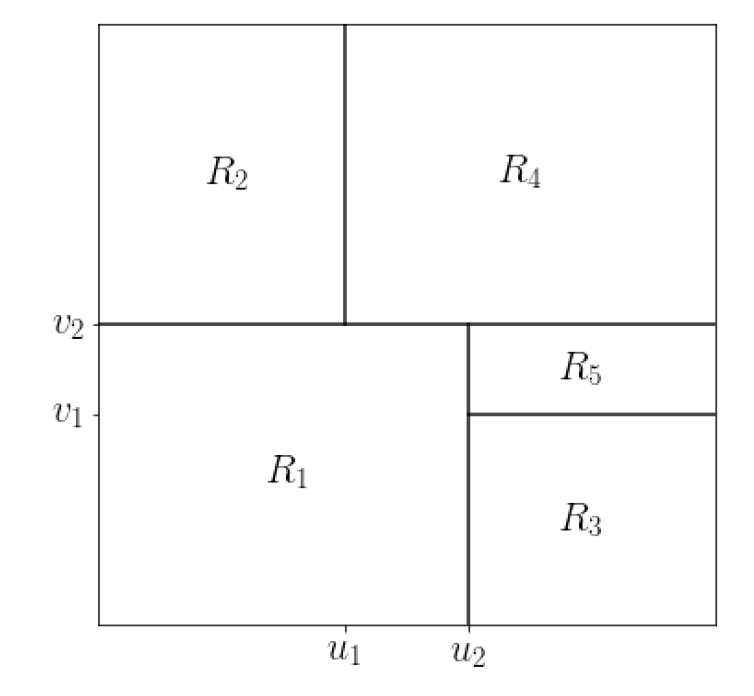
\includegraphics[width=0.5\textwidth,clip]{exemplePartition.png}
	\end{center}
	
	\bfblue{Remarque } Un arbre de décision partitionne l’espace $\X$ des observations en autant de régions qu’il a de feuilles dans l'arbre final construit
	
\end{frame}

	




%%------------------------------------------------------------------------------------------
\begin{frame}{Règle d'aggrégation}
	
	Supposons que l'algorithme a partitionné le jeu de données en $r$ régions $R_1, R_2, \dots, R_r$.\\[1em]
	
	Toutes les observations qui tombent dans une même feuille, i.e. qui appartiennent à une même région, reçoivent alors la même étiquette.\\[1em]
	
	
		\bftitle{Problème de classification} L'étiquette prédite d'un nouveau point $x$ qui est dans une région est l’étiquette majoritaire dans la région des observations d'apprentissage qui sont dans cette région
	$$ f(x) = \sum_{j=1}^r \mathbb{1}\left\{x \in R_j\right\} \, \text{arg}\,\max\limits_{k \in \{1,\dots, C\}}\,  \sum_{\substack{i \in \{1,\dots,n\} \\ x_i \in R_j} } \mathbb{1}\left\{y_i = k\right\} $$
	
	
	\bftitle{Problème de régression} L'étiquette prédite d'un nouveau point $x$ qui est dans une région est l’étiquette moyenne des observations d'apprentissage qui sont dans cette région
$$ f(x) = \sum_{j=1}^r \mathbb{1}\left\{x \in R_j\right\} \, \color{black}{\dfrac{1}{\vert R_j \vert}} \sum_{\substack{i \in \{1,\dots,n\} \\ x_i \in R_j} } y_i $$
	
	
	
	
\end{frame}


%%------------------------------------------------------------------------------------------

\begin{frame}{Variables séparatrices}
	
	\begin{center}
		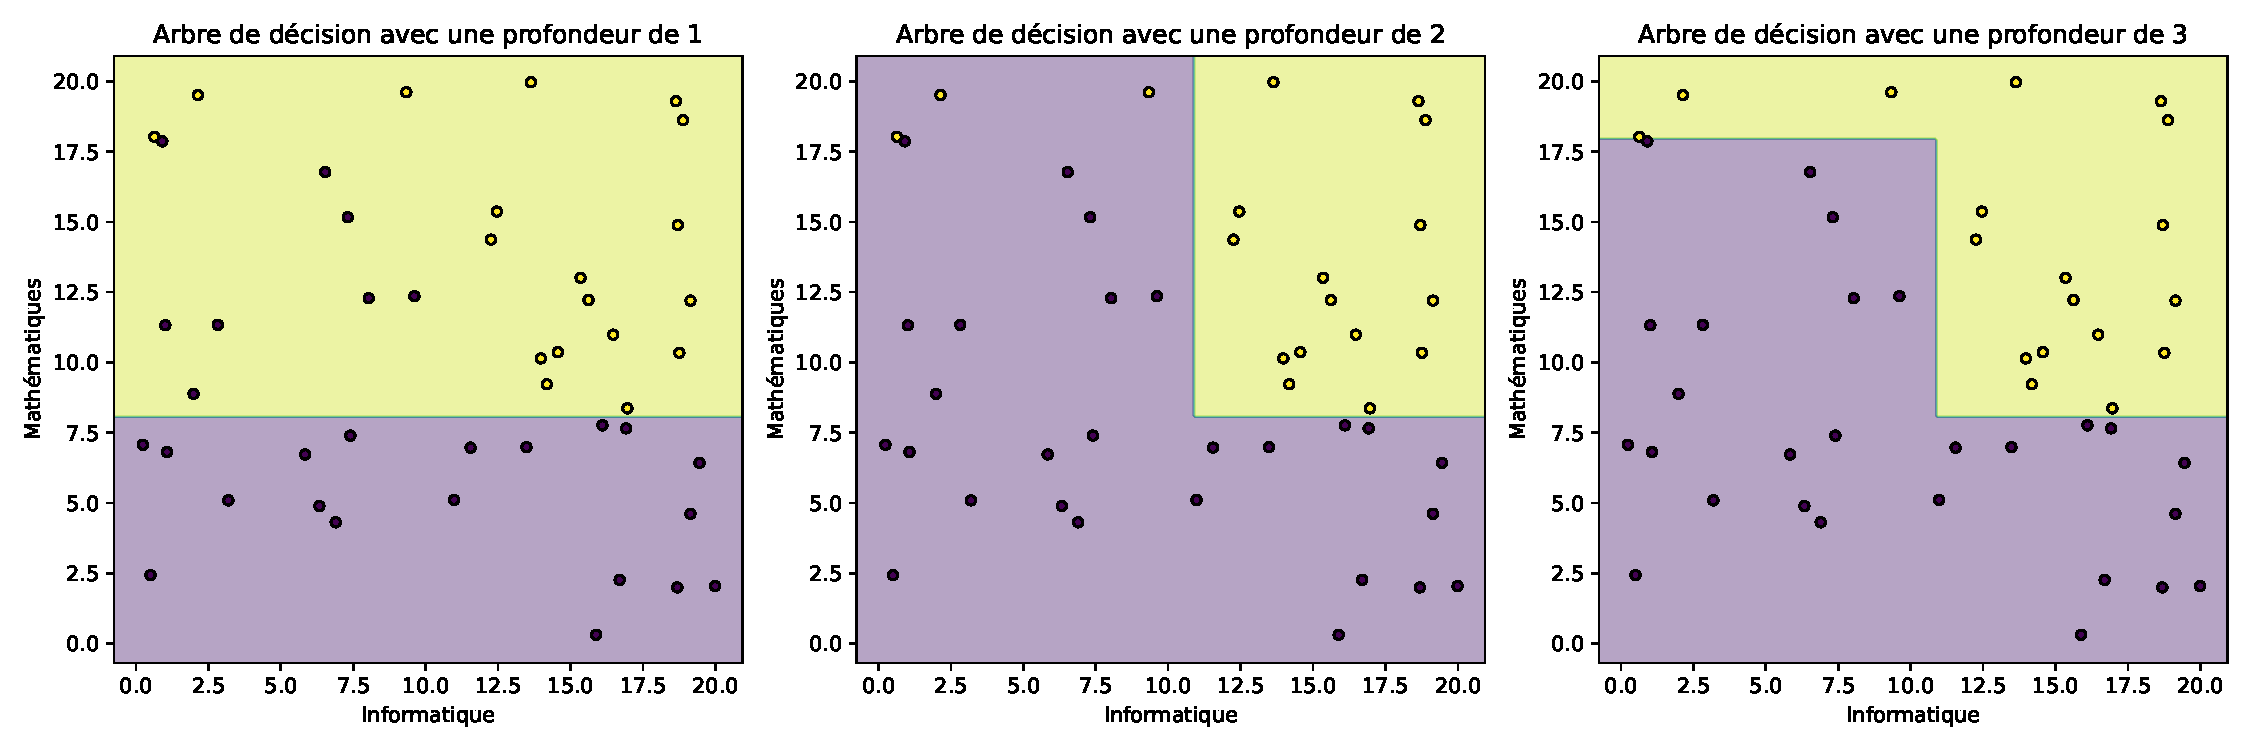
\includegraphics[width=1\textwidth,clip]{data_tree_cart.pdf}
	\end{center}
	
	\vspace*{3em}
	\begin{vblock}{}\centering
		Pour un noeud, comment choisir la bonne séparation, i.e. la bonne \textbf{variable séparatrice} et la frontière de séparation ?
	\end{vblock}
	
\end{frame}
	
%%------------------------------------------------------------------------------------------
%%------------------------------------------------------------------------------------------


\begin{frame}{Quel partitionnement - classification}

	 En classification, pour un noeud (une région $R$), on choisit le découpage qui maximise le gain d'information, i.e., on choisit la variable séparatrice $x^j$ et le seuil de séparation $seuil$ ($s$ pour une variable continue ou $\S$ pour une variable discrète) qui maximise
		
		$$\mathcal{IG}(R_l, R_m)=\mathcal{I}(R)-\frac{n_l}{n} \,\mathcal{I}\left(R_{l}(x^j, seuil)\right)-\frac{n_m}{n} \,\mathcal{I}\left(R_m(x^j, seuil)\right)$$
		
	avec
	\begin{itemize}
		\item 	$\mathcal{I}$ : un critère d'impureté qui quantifie à quel point la région considérée est « polluée » par des éléments des classes qui n’y sont pas majoritaires.\\[0.5em]
		\item  $n$ : le nombre de points $x_i$ du jeu d'entraînement qui sont dans $R$.
		\item  $n_l$, $n_m$ : le nombre de points $x_i$ du jeu d'entraînement qui sont respectivement dans $R_l$ et $R_m$
	\end{itemize}	
	% \(S\) le jeu de données associé au nœud courant, et \(S^l\) et \(S^r\) la partition (\(n, n_l, n_r\) pour la taille du jeu de données).
	
		\vspace*{3em}
	\begin{vblock}{}\centering
	 Quels critères d'impureté utiliser ?
	\end{vblock}
		
\note{dire que quand $x^j$ est continue, on ne sélectionne pas tous les seuils possibles car une infinité. Faire un exemple dans le cas variables nominales et variables continues et dire une phrase pour qu'ils comprennent comment on combine}
\end{frame}
%%------------------------------------------------------------------------------------------
%%------------------------------------------------------------------------------------------


\begin{frame}{Critères d'impureté}
	\vspace*{-1em}
	Soit  \(p_k\) est la proportion d'éléments de la classe \(k\) dans la région \(R\).\\[0.5em]
	
	\begin{itemize}
		\item \textbf{Impureté de Gini} \\
		Permet de quantifier la probabilité qu’un exemple du jeu d’entraînement soit mal étiqueté s’il était étiqueté aléatoirement en fonction de la distribution des étiquettes dans $R$
		$$\textstyle \mathcal{I}_{\mathcal{G}}(R)=\sum_{k=1}^C p_k(1-p_k) = \sum_{k=1}^C \sum_{k' \neq k \in \{1,\dots C\}} p_k p_{k'}$$
		
		\vspace*{-0.5 em}
		\item \textbf{Entropie}\\
		Permet de définir l’impureté d’une région $R$ de sorte à choisir la séparation qui maximise le gain d’information : le but de la construction est alors de minimiser la quantité d’information supplémentaire nécessaire pour étiqueter correctement les exemples d’entraînement de $R$.
	$$ \textstyle \mathcal{I}_\mathcal{E}(R)=-\sum_k p_k \text{log}_2( p_k)$$

		\item \textbf{Erreur de classification} \\
		Permet de définir l’impureté d’une région $R$ comme la proportion d’exemples de cette région qui n’appartiennent pas à la classe majoritaire.
		 $$\mathcal{I}_{EC}(R)=1-\text{max}_k(p_k)$$
	\end{itemize}

\note{faire exemple impureté Gini pour comprendre que quand un peu de chaque classe, pas bon + voir entropie}
\end{frame}
%%------------------------------------------------------------------------------------------

\begin{frame}{Quel partitionnement - régression}
	\begin{itemize}
		\item Soit le \textit{Mean-Squared Error} MSE (relativement à la moyenne) : 
		\[\text{MSE}(R)=\frac{1}{n}\sum_i (y_i-\bar{y})^2\]
		\item On cherche à minimiser le critère suivant\,:
		\[\frac{n_l}{n}\text{MSE}(R_l)+\frac{n_r}{n}\text{MSE}(R_m)\]
		\item On calcule le MSE relativement à la moyenne car celle-ci est justement notre prédiction pour un nœud fixé.
	\end{itemize}
	
\end{frame}

%%------------------------------------------------------------------------------------------


\begin{frame}{Sélection de l'arbre}
	
	\begin{vblock}{}\centering
	Quand est-ce qu'on arrête la construction d'un arbre ?
\end{vblock}
	
	
	\vspace*{2em}
	\begin{itemize}
		\item Si l'arbre est peu profond, on risque de mal modéliser le problème (sous-apprentissage)\\[1em]
		\item Si l'arbre est trop profond, on risque de "trop coller aux données" et donc de sur-apprendre
	\end{itemize}
\end{frame}

%%------------------------------------------------------------------------------------------

\begin{frame}{Sélection de l'arbre }
	
\bftitle{	Stratégie n°1 }\\[2em]

On détermine un des hyper-paramètres suivant par validation
croisée\\[1em]

\begin{itemize}
	\item Profondeur maximale\\[0.5em]
	\item nombre de feuilles maximal\\[0.5em]
	\item nombre d’exemples minimal dans une feuille/nœud
\end{itemize}
\vspace*{2em}
Question : comment se comporte la variance et le biais en fonction de la profondeur de l'arbre ?
\vspace*{2em}
\end{frame}

%%------------------------------------------------------------------------------------------

\begin{frame}{Sélection de l'arbre }
	
	\bftitle{	Stratégie n°2 - Élagage }\\[2em]
	
	On utilise un ensemble de validation pour re-visiter un arbre appris
	sans limite sur un ensemble d’apprentissage. On ne garde que les
	branches qui apportent une amélioration en validation. \\[1em]
	
	C'est une méthode de régularisation permettant de contrôler la complexité de l’arbre, mesurée par le nombre de régions qu’il définit. En particulier, on cherche à minimiser le coût en complexité suivant d'un arbre T :
	
	$$C_\lambda(T) = \sum_{l=1}^{|T|} n_l \,  \I\left(R_l\right) + \lambda |T| $$
	
	où
	\begin{itemize}
		\item $|T|$ est le nombre de régions définies par l'arbre $T$\\[0.5em]
	\item $\lambda>0$, un hyperparamètre permettant de contrôler l’importance relative de la mesure d’erreur et de la complexité
\end{itemize}


\end{frame}

%%------------------------------------------------------------------------------------------
\begin{frame}
	
	\vspace*{4em}
		\warning \hsp Les arbres de décision ont tendance à donner des modèles trop simples et à avoir des performances de prédiction à peine supérieures à des modèles aléatoires et peu robustes aux variations dans les données. On les qualifie d’apprenants faibles (weak learners en anglais). Heureusement, il est possible d’y remédier grâce aux méthodes ensemblistes (bagging, forêts aléatoires, boosting, voir cours \textit{Régularisation et optimisation})


\end{frame}

%\begin{frame}{}
%	
%Pour une fonction $\phi : \bbR \to \Y$ choisie adéquatement, on cherche $\widehat{\mathbf{w}}$ et $\widehat{b}$  tels que
%
%$$ \left(\widehat{\mathbf{w}},\widehat{b}\right)= \text{{arg}}\,\min\limits_{\mathbf{w} \in \bbR^d \, b \in \bbR}\, \dfrac{1}{n}  \displaystyle \sum_{i=1}^n \ell\ \left(y_i, \phi\left( \langle {\mathbf{w}},x_i \rangle + b\right) \right)$$
%
%avec $\H_\phi := \left\{\mathbf{x}\mapsto \phi  \ \circ \ h_{\mathbf{w},b}  (\mathbf{x}), \hsp  h_{\mathbf{w},b} \in L_d\right\}$
%	
%	\begin{center}
%		La régression logistique consiste à résoudre le problème de minimisation lorsque $\ell$ est le coût 
%	\end{center}
%
%\end{frame}
%%------------------------------------------------------------------------------------------
%
%%\subsection{Classifieurs Linéaires\\[0.5em] --\\[0.5em]  Le coût quadratique}
%%
%%\subsection{Classifieurs Linéaires\\[0.5em] --\\[0.5em]  Le coût logistique}
%
%\subsection{Classifieurs Linéaires\\[0.5em] --\\[0.5em]  Évaluer un modèle avec l'AUC}
%
%\subsection{Classifieurs Linéaires\\[0.5em] --\\[0.5em]  Classification Multiclasse}
%
%
%	



\begin{frame}{Références}
	\begin{thebibliography}{2}
			\vspace{-1.8em}
			
	%	\bibitem{1} L.~Bel, J.N.~Bacro and C.~Lantuéjoul, \textcolor{black}{Assessing extremal dependence of environmental spatial fields,} \emph{Environmetrics}, 19(2):163-182, 2008
		
		\bibitem{pouet} C.A.~Azencot \textcolor{black}{{\href{http://cazencott.info/dotclear/public/lectures/IntroML_Azencott.pdf}{Introduction au Machine Learning}}}, \emph{Dunod},\\ ISBN : 978-2-10-084143-1\\[2em]
		
	%	\bibitem{CNP2006} D.~Cooley, P.~Naveau and P.~Poncet \textcolor{black}{Variograms for spatial max-stable random fields}, pages 370-390, \emph{Springer New-York}, 2006
		
		\bibitem{2} S.~Shalev-Shwartz and S.~Ben-David, \textcolor{black}{Understanding Machine Learning: From Theory to Algorithms,} \emph{Cambridge University Press}, DOI : 10.1017/CBO9781107298019, 2014\\[2em]
		%
	%	\bibitem{3} C.~Dombry, S.~Engelke, M.~Oesting (2016) \textcolor{black}{Exact simulation of max-stable processes}, \textit{Biometrika} 103(2):303–317
		
		\bibitem{E} T.~Hastie, R.~Tibshirani, and J.~Friedman. \textcolor{black}{The Elements of Statistical Learning}, \emph{Springer New York}, DOI : 10.1007/978-0-387-84858-7, 2009
		
		
		%
		%	\bibitem{4} R.A.~Fisher and L.H.C.~Tippett, \textcolor{black}{Limiting forms of the frequency distribution of the largest or smallest member of a sample,} \emph{Mathematical Proceedings of the Cambridge Philosophical Society}, 24(2):180-190, 1928\\[0.3em]
		%	
	\end{thebibliography}
	
\end{frame}
\end{document}
